\documentclass[12pt]{article}
\usepackage{geometry}
\usepackage{amsfonts, epsfig}
\usepackage{amsmath}
\usepackage{wrapfig} % for wrapping text around figures and tables
\usepackage{graphicx}
\usepackage{multirow}
\usepackage{fancyhdr}
\usepackage{booktabs} % for better table rules
\usepackage{caption} % to customize caption format
\usepackage{linegoal} % for determining the remaining width of the line
\usepackage[backend=biber, sorting=none]{biblatex}
\usepackage{subcaption}

% reference file
\addbibresource{report.bib}

\geometry{
    left=20mm,
    right=20mm,
    top=20mm,
    bottom=20mm
}

% header and footer
\makeatletter
\def\@oddhead{\parbox{\textwidth}{\raggedright\sffamily\underline{\texttt{Question 1 - Visualization and analysis of the Palmer penguin dataset}} \hfill \thepage}}
\def\@oddfoot{\parbox{\textwidth}{\raggedright\footnotesize\texttt{emamtm0067.github.io} / \texttt{ematm0044.github.io}}}
\makeatother

% Redefine the table and figure formats to bold
\captionsetup[table]{labelfont=bf}
\captionsetup[figure]{labelfont=bf}
\captionsetup{font=small}

\begin{document}
\begin{center}
\subsection*{Q1 - Visualization and analysis of the Palmer dataset}
\end{center}

\begin{wraptable}{r}{0.5\textwidth} % {alignment}{width}
  \small
  \begin{center}
  \vspace{-1.5\baselineskip} % Remove space before the table
  \setlength{\abovecaptionskip}{5pt}
  \setlength{\belowcaptionskip}{5pt}
  \fontsize{10}{10}\selectfont % Change font size here
  \begin{tabular}{l|l|l}
  Attribute&Type&Values in the dataset\\
  \hline
  species&categorial&Adelie, Chinstrap, Gentoo\\
  island&categorial&Torgersen, Biscoe, Dream\\
  bill length&numerical&32.1mm - 59.6mm\\
  bill depth&numerical&13.1mm - 21.5mm\\
  flipper length&numerical&172mm - 231mm\\
  body mass&numerical&2700g - 6300g\\
  sex&categorial&Male, Female
  \end{tabular}
  \vspace{-1.5\baselineskip} % Remove space before title
  \end{center} 
  \caption{Attributes of the Palmer penguin dataset}
  \vspace{-1\baselineskip} % Remove space after the table
  \label{tab:dataset}
\end{wraptable} 

\noindent
The Palmer penguin dataset consists of 344 records of the physical attributes of three species of penguin 
living on three islands in Antarctica (Table~\ref{tab:dataset}) \cite{PM}. 
In this report, consideration is given to data cleaning and preparation, 
the dataset is explored through visualization and analysis is carried out 
to compare the accuracy performances of a small number of AI approaches. 

\vspace{\baselineskip}
\subsection*{Data cleaning - missing values, standardization and data imbalance}

\begin{wrapfigure}{r}{0.5\textwidth} % {alignment}{width}
  \centering
  \vspace{-0.5\baselineskip} % Remove space before the table
  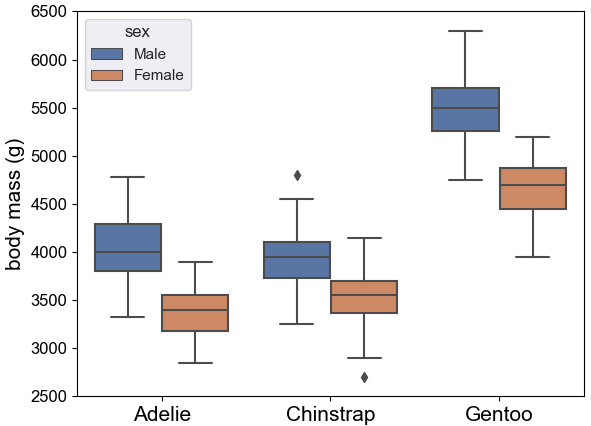
\includegraphics[width=0.48\textwidth]{sex.png} % Adjust the width as needed
  \vspace{-0.5\baselineskip} % Remove space before title
  \caption{All numerical features show a significant statistical difference between the male and female measurements, as seen in the body mass boxplot above. Shown are median values, Q1 and Q3 quartiles, as well as outliers that are outside the range Q1-1.5IQR to Q3+1.5IQR, where IQR=Q3-Q1.}
  \vspace{-0.5\baselineskip} % Remove space before title
  \label{fig:sex}
\end{wrapfigure}   

Two of these records can be deleted immediately as they are missing 
values for all of the numerical attributes and the sex feature 
and any imputation is unlikely to be reliable. 
The remaining nine records have no value only for the sex attribute. 
As can be seen in Figure~\ref{fig:sex}, the physical attributes of the male and female of each species 
are statistically different and so it is reasonable to consider assigning a sex 
to those records missing this attribute. Following standardization, 
a Shapiro-Wilk test was performed to confirm each numerical attribute exhibits a normal distribution \cite{shapiro1965analysis} 
and Z-tests were performed to assess separately both the 
hypothesis that the missing sex value is male and that it is female \cite{freedman2007statistics}. 
It was found that two of the records could be imputed as male and three as female 
and these were then retained in the dataset. 
The remaining four records were removed from the dataset. 
The cleaned dataset consisted of 338 records made up of 147 Adelie penguins 
(74 male, 73 female), 68 Chinstrap penguins (34 male, 34 female) and 123 Gentoo penguins (62 male, 61 female).

A number of the methods applied in this work involve distance measures 
and so may be biased in favour of features with smaller standard deviations \cite{hastie2009elements}. 
This bias can be removed by standardizing the four numerical attributes independently 
(to give zero mean and unity standard deviation). 
Standardization uses only the statistics of training sets, 
but standardization is also applied to test sets. If a dataset is imbalanced, 
AI approaches may be biased in predicting classes that are more commonly found in the training data. 
The Palmer penguin dataset is somewhat imbalanced, 
with the number of Chinstrap records being around half of that of either Adelie or Gentoo, 
which are present in similar numbers. 
The importance of imbalance depends on the analysis method applied. 
It is known that all the methods adopted in the current work are generally little affected by imbalanced data \cite{he2009learning} 
and so no modifications were made to reduce imbalance.

\begin{wrapfigure}{r}{0.5\textwidth} % {alignment}{width}
  \centering
  \vspace{-0.5\baselineskip} % Remove space before the table
  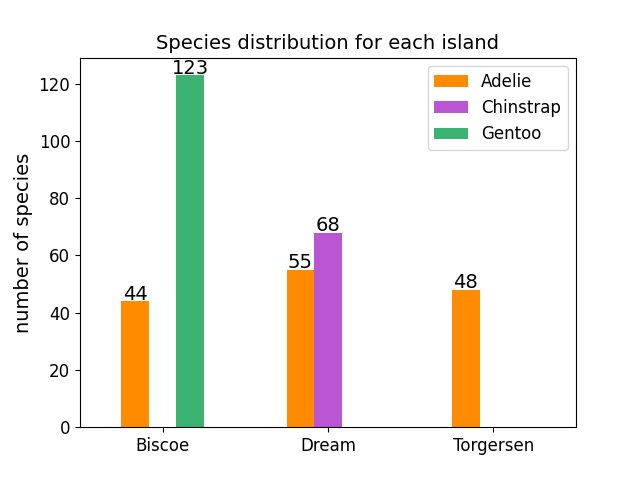
\includegraphics[width=0.48\textwidth]{islands.png} % Adjust the width as needed
  \vspace{-0.5\baselineskip} % Remove space before title
  \caption{All numerical features show a significant statistical difference between the male and female measurements, as seen in the body mass boxplot above. Shown are median values, Q1 and Q3 quartiles, as well as outliers that are outside the range Q1-1.5IQR to Q3+1.5IQR, where IQR=Q3-Q1.}
  \vspace{-0.5\baselineskip} % Remove space before title
  \label{fig:islands}
\end{wrapfigure}

\vspace{\baselineskip}
\subsection*{Visualization of the dataset}

Figure~\ref{fig:islands} shows the species distribution across the three islands in the study. 
Chinstrap and Gentoo penguins are found only on one island, so island is a potential confounding factor, 
possibly affecting physical characteristics due to environmental factors (such as predators or food supply). 
A Shapiro-Wilk test was used to confirm that the numerical features of the Adelie penguins (that are found on 
all the islands) are normally distributed and an ANOVA test confirmed that their physical characteristics are not significantly influenced by the island inhabited. 
Consequently, it was considered unlikely that the island is a confounding factor in the dataset.

\begin{wrapfigure}{r}{0.6\textwidth} % {alignment}{width}
  \centering
  \vspace{-0.3\baselineskip} % Remove space before the table
  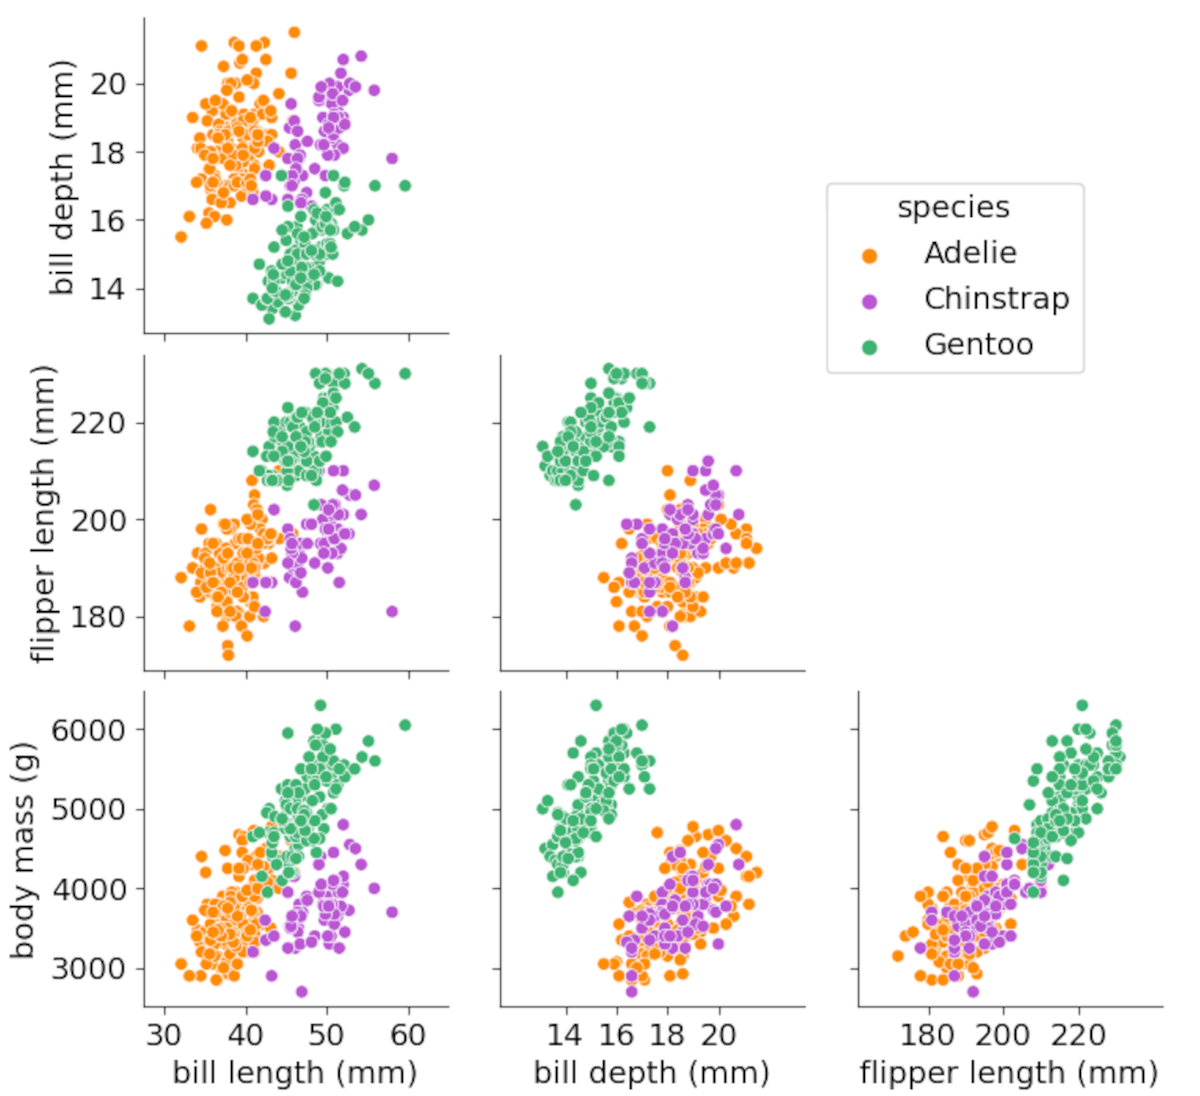
\includegraphics[width=0.58\textwidth]{pairwise.png} % Adjust the width as needed
  \vspace{-0.5\baselineskip} % Remove space before title
  \caption{All numerical features show a significant statistical difference between the male and female measurements, as seen in the body mass boxplot above. Shown are median values, Q1 and Q3 quartiles, as well as outliers that are outside the range Q1-1.5IQR to Q3+1.5IQR, where IQR=Q3-Q1.}
  \vspace{-0.5\baselineskip} % Remove space before title
  \label{fig:pairwise}
\end{wrapfigure}

Pairwise scatterplots for the numerical features are shown in Figure~\ref{fig:pairwise}. 
It can be seen that bill depth in combination with either flipper length or body mass 
yields a separable cluster of Gentoo penguins (shown in green) allowing them to be identified. 
No pairwise combination of numerical features completely separates Adelie (orange) from Chinstrap (purple) clusters, 
but good separation is provided in the distributions involving bill length, 
making this a candidate feature for distinguishing between these species.  

Figure~\ref{fig:sex} above shows there is a difference in the body masses of the male and female samples for each of the three species. 
Differences between the sexes for the other three numerical physical characteristics in the dataset were also apparent. 
Since narrower distributions are apparent if the sex of the species is considered rather than just the species itself, 
including sex is likely to provide a finer grained distinction for species classification 
and this knowledge can be used to improve performance, as discussed in the analysis section below. 

\subsection*{Implementation}

All code was written in Python 3.11 \cite{python311} using ‘Scikit-Learn’ libraries \cite{scikit-learn} running under Ubuntu Linux \cite{ubuntu}. 
The code is available in a Gitub repository \cite{TimAIRepo}. Predicting the penguin species from the given features is a classification problem. 
Results are obtained from a baseline method, two convention classification approaches, 
namely k-Nearest Neighbour (knn) \cite{bishop2006pattern} and random forest \cite{breiman2001random}, 
unsupervised k-means (following cluster labelling) \cite{tan2005introduction} and a novel combined visualization and analysis (CVA) approach 
introduced here that uses insights from visualizations combined with two-dimensional linear Support Vector Machines (SVMs) classification.

\begin{wraptable}{r}{0.7\textwidth} % {alignment}{width}
  \small
  \begin{center}
  \vspace{-1.5\baselineskip} % Remove space before the table
  \setlength{\abovecaptionskip}{5pt}
  \setlength{\belowcaptionskip}{5pt}
  \fontsize{10}{10}\selectfont % Change font size here
  \begin{tabular}{l|l|l}
  Method & Metaparameters & Values considered\\
  \hline
  \multirow{3}{*}{knn} & number of nearest neighbours k	  & {\normalsize\textbf{1}}, 2, 3, 4, 5, 6, 8, 10 \\
                        & weight function for prediction	& {\normalsize\textbf{uniform}}, distance \\
                        & distance metric for neighbours	& {\normalsize\textbf{Manhattan}}, Euclidean \\
  \hline
  \multirow{5}{*}{random forest} & number of trees in the forest	 & 5, {\normalsize\textbf{10}}, 15, 20, 25 \\
                                  & maximum depth of trees	       & {\normalsize\textbf{no maximum}}, 10, 20 \\
                                  & minimum samples to split node	 & {\normalsize\textbf{2}}, 5, 10 \\
                                  & minimum samples at leaf node   & {\normalsize\textbf{1}}, 2, 4 \\
                                  & function for quality of split  & {\normalsize\textbf{gini}}, entropy \\
  \hline
  \multirow{4}{*}{k-means} & number of clusters k                & 2, {\normalsize\textbf{3}}, 4, 5, 6, 7, 8, 9, 10 \\
                            & centroid initialization method     & {\normalsize\textbf{k-means++}}, random \\
                            & number of runs for centroid seeds	 & 2, {\normalsize\textbf{5}}, 10, 20 \\
                            & maximum number of iterations       & 5, {\normalsize\textbf{10}}, 20, 50 \\
  \hline
  \multirow{3}{*}{CVA} & regularization parameter (C)  & 0.1, 1, {\normalsize\textbf{10}}, 100 \\
                        & kernel coefficient (gamma)   & {\normalsize\textbf{1}}, 0.1, 0.01, 0.001 \\
                        & kernel type                  & rbf, {\normalsize\textbf{linear}}, polynomial \\
  \hline
  \end{tabular}
  \vspace{-1.5\baselineskip} % Remove space before title
  \end{center} 
  \caption{Metaparameters considered in training the methods. 
  The values shown in bold are those that most consistently produced results of 
  best accuracy during validation and so were selected for generating results}
  \vspace{-1\baselineskip} % Remove space after the table
  \label{tab:metaparameters}
\end{wraptable} 


For all the methods implemented, 20\% of the dataset was kept for a test set. 
To reduce the potential for overfitting, the classification methods (all but k-means) were trained using ‘holdout validation’, 
where the remaining 80\% of the dataset was used in a five-fold cross-validation configuration \cite{james2013introduction}. For all methods, 
the Scikit-Learn function GridSearchCV was employed to tune metaparameters \cite{scikit-learn}. 
Table~\ref{tab:metaparameters} shows the values selected for the metaparameter grid for each of the AI methods 
and those values that gave best performance were selected to obtain the accuracy results from the test set. 
Scikit-Learn includes pseudo-random procedures for selecting validation and test set values and 100 of these were used 
both when selecting metaparameters and when deriving accuracy results.

\subsection*{Results and analysis}

\begin{wraptable}{r}{0.6\textwidth} % {alignment}{width}
  \small
  \begin{center}
  \vspace{-1.5\baselineskip} % Remove space before the table
  \setlength{\abovecaptionskip}{5pt}
  \setlength{\belowcaptionskip}{5pt}
  \fontsize{10}{10}\selectfont % Change font size here
  \begin{tabular}{l|l}
  Method & Accuracy\\
  \hline
  baseline, most numerous species & 43.49\% \\
  \hline
  kNN, all features	& 99.24\% \\
  kNN, no island &	99.46\% \\
  \hline
  random forest, all features	& 98.57\% \\
  random forest, no island, flipper length or body mass	& 98.57\% \\
  \hline
  k-means, all numerical features & 97.06\% \\
  k-means, separate clusters for each sex & 98.23\% \\
  \hline
  CVA using bill depth, flipper length, bill length	& 98.56\% \\
  CVA using bill depth, flipper length, bill length, sex &98.78\% \\
  \hline
  \end{tabular}
  \vspace{-1.5\baselineskip} % Remove space before title
  \end{center} 
  \caption{Mean classification accuracy from 100 test sets each generated by a pseudo random approach 
  and using the parameters identified in Table~\ref{tab:metaparameters}}
  \vspace{-1\baselineskip} % Remove space after the table
  \label{tab:results}
\end{wraptable} 

The results in Table~\ref{tab:results} include a baseline that is used to demonstrate performance improvements achieved by the AI methods being considered. 
If the performance cannot be improved significantly compared to the baseline, 
this may indicate that the method is not suitable or that the problem itself is particularly intractable. 
In classification, the baseline method is often simply to select the most frequent class in the observations and, 
in this work, this is the Adelie penguins, giving an accuracy of 43.49\% (147/338).

\textbf{Classification method 1 - knn}  
The performance of knn was found to be improved by omitting features from training. 
An exhaustive search involving omitting all combinations of features in turn determined that the best accuracy was obtained 
when island was omitted and this occurred when k=3. It appears that island was not providing any additional information 
and the higher value of k implies better generalization may have been achieved.

\textbf{Classification method 2 - Random forest}  
Including all of the features in the analysis provided an accuracy marginally better 
than could be achieved using knn when its features were carefully selected. 
No performance improvement was found by using fewer features, indicating that, for the Palmer penguin dataset at least, 
it requires considerably less implementation effort to achieve good performance using a random forest than it does using knn. 
A marginal improvement in performance was apparent when island, flipper length or body mass were not included in training.

\begin{wrapfigure}{r}{0.5\textwidth} % {alignment}{width}
  \centering
  \vspace{-0.5\baselineskip} % Remove space before the table
  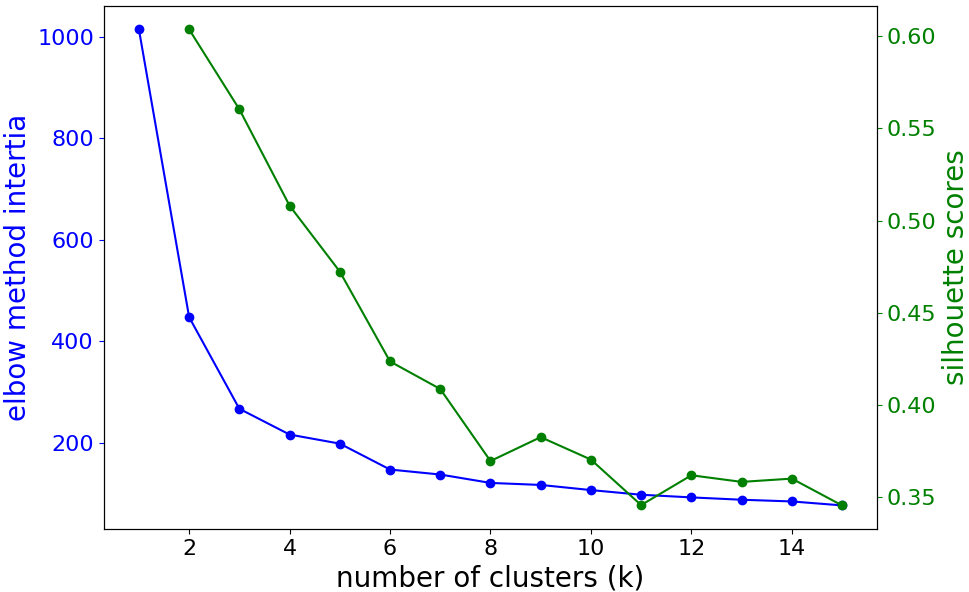
\includegraphics[width=0.48\textwidth]{kmeansvalue.png} % Adjust the width as needed
  \vspace{-0.5\baselineskip} % Remove space before title
  \caption{To estimate k for k-means, the elbow method uses the change in slope of ‘inertia’ (here k=3) and the silhouette method uses the score closest to 1 (here k=2)}
  \vspace{-0.5\baselineskip} % Remove space before title
  \label{fig:kmeansvalue}
\end{wrapfigure}

\textbf{Unsupervised method - k-means}  
Although an unsupervised clustering method, 
k-means can be used for classification by matching clusters with classes. 
Only numerical features were included in the k-means analysis as it is not able to deal 
with unordered categorical data either directly or by labelling. 
The number of clusters (k) was selected using both the elbow and silhouette methods, 
giving values of k=3 and k=2 respectively, as shown in Figure~\ref{fig:kmeansvalue}. 
However, in practice it was found that accuracy improved significantly when k > 3 
and this was probably due to the fact that, for smaller values of k, 
clusters were not always formed for all three species. 
Figure~\ref{fig:kmeansmap} illustrates the mapping of classes to clusters using two feature dimensions. 
No improvement in accuracy was obtained by reducing the number of features, 
but, in an additional experiment, separate sets of k-means clusters were created for each sex 
and this led to a small improvement in accuracy. 

\begin{wrapfigure}{r}{0.5\textwidth} % {alignment}{width}
  \centering
  \vspace{-0.5\baselineskip} % Remove space before the table
  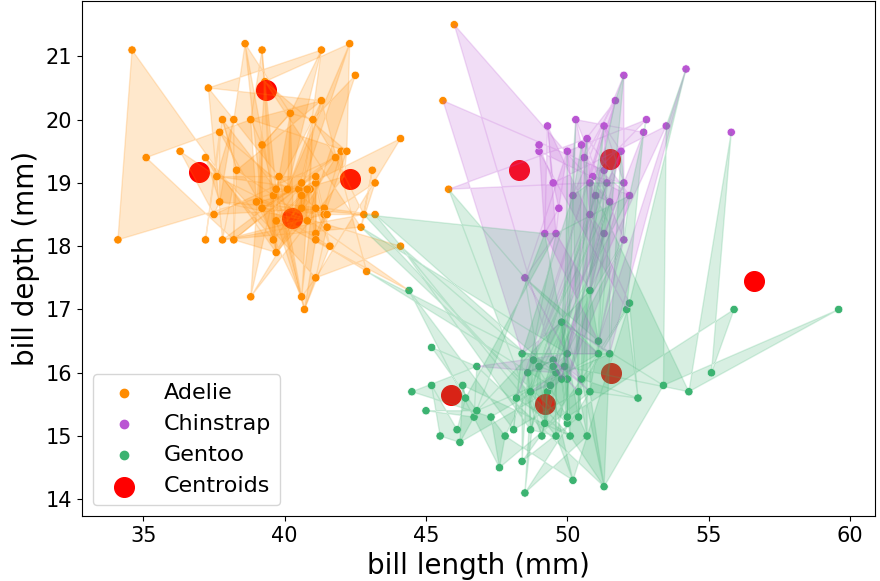
\includegraphics[width=0.48\textwidth]{kmeansmap.png} % Adjust the width as needed
  \vspace{-0.5\baselineskip} % Remove space before title
  \caption{k-means clusters mapped to species according to majority voting. Assignments to classes are shown by polygon colours (here k=10 and colouring limited to 50 samples).}
  \vspace{-0.5\baselineskip} % Remove space before title
  \label{fig:kmeansmap}
\end{wrapfigure}

\textbf{A novel combined visualization and analysis (CVA) approach}  
This work introduces the CVA approach that involves using visualizations of pairwise combinations of numerical data 
to identify a short sequence of two-dimensional linear classifiers based on SVMs. 
CVA requires greater manual effort to gain a deeper understanding of the nature of the dataset 
and this is in contrast with `black box' classification approaches that are often applied with limited knowledge 
of the method adopted and little underlying insight into the nature of the data. 
The drawbacks of the CVA approach are that it is not generally applicable as it may not always be feasible 
or possible to extract the necessary insights from visualizations, 
and that the approach will become more difficult to apply as the number of features is increased. 
In application to the Penguin data, it was found to be able to produce results of accuracy almost as good as conventional approaches.

The figure is Figure~\ref{fig:entire_figure}

\begin{figure}
  \begin{subfigure}{0.5\textwidth}
    \centering
    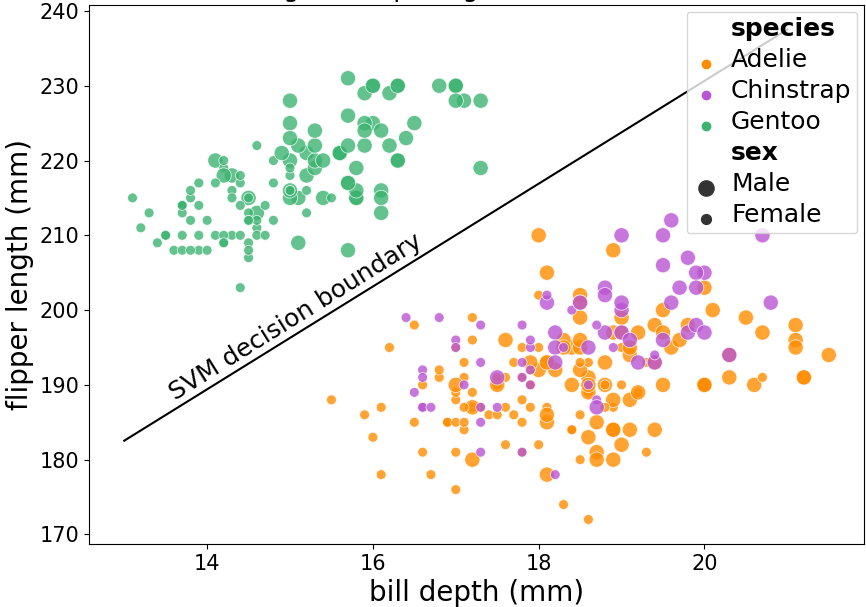
\includegraphics[width=1.05\textwidth]{sup_fliplen_billdepth.png} % Adjust the width as needed
    \caption{Caption for part (a)}
    \label{fig:part_a}
  \end{subfigure}
  \hfill
  \begin{subfigure}{0.5\textwidth}
    \centering
    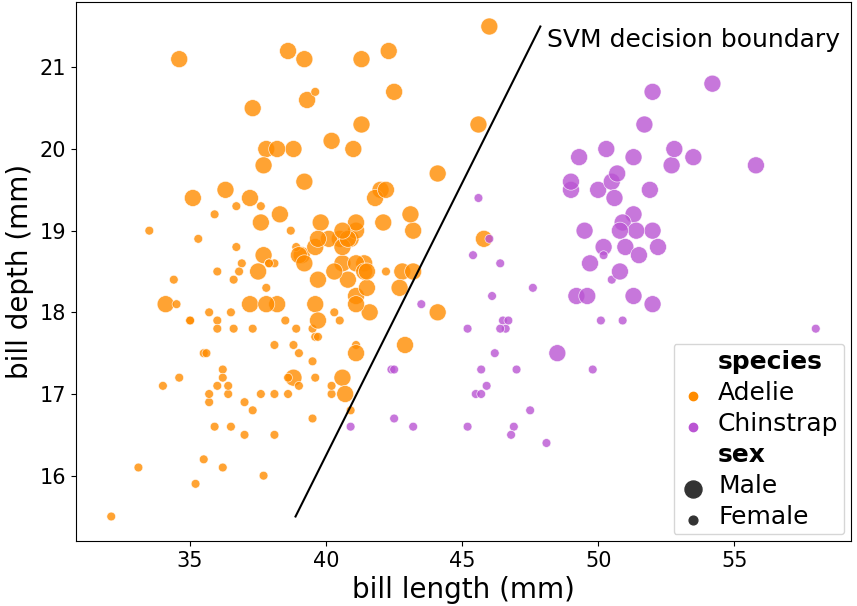
\includegraphics[width=1.05\textwidth]{sup_billlen_billdepth.png} % Adjust the width as needed
    \caption{Caption for part (b)}
    \label{fig:part_b}
  \end{subfigure}
  \caption{Overall caption for the entire figure}
  \label{fig:entire_figure}
\end{figure}

You can write in \textbf{bold}, or \textsl{italics} or \texttt{true
  type}, often the latter is used for specific commands or libraries in a
programming language, as in `I used \texttt{numpy} v1.23.4 to\ldots'. Notice the use of the left quote symbol found in the top left of the keyboard to get the left quote. There is also blackboard bold often used for things like $\mathbb{R}$ for real numbers and there is calligraphic for fancy things like $\mathcal{L}$ but this is becoming increasing irrelevant to what you are likely to need! 




\printbibliography


\end{document}
